\documentclass[11pt]{article}
\usepackage[dvipsnames]{xcolor}
\usepackage{times}
\usepackage{amsmath,amsthm,amssymb,setspace,enumitem,epsfig,titlesec,verbatim,array,eurosym,multirow}
\usepackage[sort&compress,numbers]{natbib}
\usepackage[footnotesize,bf]{caption}
\usepackage[margin=2.5cm, includefoot, footskip=30pt]{geometry}
\usepackage{standalone}
\usepackage{tikz}
\usepackage{subcaption}
\usepackage{hyperref}
\usepackage{tabularx}
\usepackage{booktabs}
\usepackage{blkarray}
\usepackage[ruled,vlined]{algorithm2e}
\smallskip % Erlaubt kleine Abstaende zwischen Paragraphen, falls es dem Seitenlayout hilft
\renewcommand{\baselinestretch}{1.15}
\usepackage{tikz}
\usetikzlibrary{arrows}
\usepackage{minitoc}
\usepackage{graphicx}
\usepackage{hyperref}
\usepackage{subcaption}
\usepackage{multirow}
\usepackage{multicol}
\usepackage{standalone}

\newcommand{\nikoleta}[1]{\textcolor{orange}{\textbf{NG}: #1}}
\newcommand{\christian}[1]{\textcolor{blue}{\textbf{CH}: #1}}

\def\wsls{\texttt{WSLS}}
\def\tft{\texttt{TFT}}
\def\gtft{\texttt{GTFT}}
\def\allc{\texttt{ALLC}}
\def\alld{\texttt{ALLD}}
\def\alt{\texttt{Alternator}}



\titleformat{\section}{\sffamily \fontsize{12}{15}\bfseries}{\thesection}{0.4em}{}
\titleformat{\subsection}{\sffamily\fontsize{11}{15}\bfseries}{\thesubsection}{0.4em}{}




\title{\bfseries \sffamily \Large Conditional coperation with longer memory}

%% Perhaps: Better title (Conditional cooperation with longer memory) %% 

\author{Nikoleta E. Glynatsi$^{1,*}$, Martin Nowak$^2$, Christian Hilbe$^1$\\[0.3cm]
$^{\rm 1}$Max Planck Research Group on the Dynamics of Social Behavior,\\ Max Planck Institute for Evolutionary Biology, Pl\"{o}n, Germany \\
$^{\rm 2}$Department of Mathematics,
Department of Organismic and Evolutionary Biology,\\ Harvard University, Cambridge, USA\\
$^*$To whom correspondence should be addressed. E-mail: glynatsi@evolbio.mpg.de
}
\date{}

\begin{document}

\maketitle

~\\[0.5cm]
\noindent
{\bf 
Repeated games enable evolution of cooperation if players use conditional
strategies that depend on previous interactions. A well known strategy set is
given by reactive strategies, which respond to the co-player's previous move.
Here we extend reactive strategies to longer memories. A reactive-$n$ strategy
takes into account the sequence of the $n$ last moves of the co-player. A
reactive-$n$ counting strategy takes into account how often the co-player has
cooperated during the last $n$ round. We characterize all partner strategies among
reactive-2 and reactive-3 strategies as well as among reactive-$n$ counting
strategies. Partner strategies are those that ensure mutual cooperation without
exploitation. We perform evolutionary simulations and find that longer memory
increases the average cooperation rate for reactive-$n$ strategies but not for
reactive counting strategies.
}\\[1cm]


\noindent
{\it Keywords:} Evolutionary game theory, direct reciprocity, evolution of cooperation, prisoner's dilemma



\clearpage
\newpage

\noindent
{\bf Significance statement.}

~\\[1cm]

\section*{Introduction}

The emergence of cooperation in social interactions can be explained by the
concept of direct reciprocity, where individuals assist each other through
repeated encounters~\cite{axelrod:AAAS:1981, nowak:Science:2006, sigmund2010}.
The framework commonly used to model these interactions is the Prisoner's
Dilemma. In this model, two participants, referred to as players, engage in a
series of repeated interactions. During each interaction, they must decide
whether to cooperate or defect. Cooperation typically results in more favorable
outcomes for both players, but the self-interest of each individual often leads
to a temptation to defect.

Strategies in the repeated Prisoner's Dilemma can vary in complexity. Some
strategies are straightforward, including zero-memory strategies like ALLC and
ALLD, as well as memory-1 strategies such as Tit For
Tat~\cite{axelrod:AAAS:1981} and Win Stay Lose Shift~\cite{nowak:Nature:1993}.
On the other hand, some strategies are more sophisticated, considering multiple
past interactions or additional information, such as the history of defections
by both players~\cite{harper:PLOSONE:2017, knight:PLOSONE:2018,
li:NatureCompSci:2022}.
Empirical evidence supports the idea that humans do not typically employ
zero-memory strategies; instead, they tend to favor conditional cooperation
strategies~\cite{fischbacher:AER:2010, rand:Elsevier:2013,
grujic:ScientificReports:2014}. However, when it comes to the memory size of strategies used
by humans, there is conflicting evidence. Some studies suggest that many human
strategies align with those based solely on the most recent
interaction~\cite{engle:ET:2006, dal:AER:2011, camera:GEB:2012, bruttel:TD:2012}.
Nonetheless, there is also evidence of strategies that
take into account more than just the previous round~\cite{fudenberg:AER:2012, romero:EER:2018}.

Theoretical models have primarily focused on memory-1
strategies~\cite{nowak:Nature:1993, nowak:Nature:1992, glynatsi:scientific:2020, press:PNAS:2012,
stewart:scientific:2016, kraines:elsevier:2000,
imhof:ProceedingsB:2010, baek:scientific:2016, hilbe:PNAS:2013,
chen:PNASnexus:2023, hilbe:Nature:2018, akin:EGADS:2016} due to their
mathematical tractability. This is because memory-1 strategies can be described
by four parameters, specifically, the probabilities of cooperating after each
possible outcome of the last round. Previous work has explored the entire space
of memory-1 strategies and characterized when strategies are Nash equilibria.
Furthermore, previous work has uncovered other interesting properties of these
Nash strategies. Examples include zero-determinant strategies, which constitute
a set of strategies capable of enforcing a linear relationship between the
payoffs of the two players~\cite{press:PNAS:2012}, equalizers, a set of
strategies that equalize the co-player's score, assigning it a predetermined
value independent of the co-player's strategy~\cite{hilbe:PNAS:2013}, and
partner strategies, which ensure mutual cooperation without
exploitation~\cite{hilbe:Nature:2018}.

There have been efforts to expand these findings into strategy sets with
greater memory. In the study by~\cite{ueda:RSOP:2021}, they explore
zero-determinant strategies within the context of
memory-two strategies. Meanwhile,~\cite{hilbe:PNAS:2017} delve into cooperative
strategies applicable to memory-2 and memory-3. Despite the complexity, they
successfully demonstrate that a specific set of strategies can be classified as
Nash, effectively pinpointing locations within the strategy space.
Working with higher memory strategies is not a trivial matter. Memory-1
strategies are defined by four parameters, but in the case of memory-2, one must
consider 16 parameters, and 256 parameters in the case of memory-three. Thus, the
space of strategies expands exponentially, making it challenging to derive
analytical results.

Herein, we approach higher memory strategies by focusing on a specific set of
memory$-n$ strategies that respond exclusively to one player's actions. Two such
sets exist. The first comprises reactive strategies, which solely take into
account the co-player's actions in previous turns. The second is the set of
self-reactive strategies, which consider the focal player's actions. It can be
easily demonstrated that in the case of self-reactive strategies, the Nash
equilibrium is consistently one of always defecting. Consequently, our focus is
directed toward reactive strategies.

Using reactive strategies, we can characterize partner strategies for both
reactive-2 and reactive-3 strategies. For a particular class of reactive
counting strategies, which involve counting cooperations rather than remembering
the actual actions, we can identify partner strategies across all memory
lengths. We establish this series of results by relying on a central finding: if
a player employs a reactive strategy, then the co-player using a memory-$n$
strategy can switch to a self-reactive-$n$ strategy without altering the
resulting payoffs. To assess the evolutionary properties of partner strategies,
we conduct simulations of an evolutionary process. Our findings indicate that
partner strategies are prevalent within the population, and they exhibit a
higher likelihood of evolution compared to other strategies. Moreover, we
observe that cooperation rates increase as the memory size grows.
When it comes to counting strategies, the advantages of increased
memory are rather limited. Partner strategies do not see a higher selection
frequency, and the overall cooperation rate within the population remains
almost the same.

\section*{Results}

\textbf{Definitions.}
We consider an infinitely repeated game with two players, player 1 and player 2.
In each round players can choose to cooperate ($C$) or to defect ($D$). If
both players cooperate, they receive a payoff $R$ (the reward for mutual
cooperation), and if both players defect, they receive a payoff $P$ (the
punishment for mutual defection). If one player cooperates, the cooperative
player receives the sucker's payoff $S$, and the defecting player receives the
temptation payoff $T$. We assume that the payoff are such that $T > R > P > S$
and $2 R > T + S$. This game is known as the Prisoner's Dilemma. Here, we employ
a specific parametrization of the Prisoner's Dilemma, where cooperation implies
incurring a cost $c$ for the co-player to derive a benefit $b > c$.
Consequently, the payoffs are defined as follows: \(R = b - c, S = -c, T = b, P
= 0\). In the Supplementary Information, we show that our main results
are applicable to the general Prisoner's Dilemma.

We assume in the following, that the players' decisions only depend on the
outcome of the previous $n$ rounds. To this end, an {\it $n$-history for player
$i \in \{1, 2\}$} is a string $h^i=(a^i_{-n},\ldots,a^i_{-1})\!\in\!\{C,D\}^n$
where an entry $a^i_{-k}$ corresponds to player $i$'s action $k$ rounds ago. Let
$H^i$ denote the space of all $n$-histories for player $i$ where set $H^i$
contains $|H^i|=2^{n}$ elements. A {\it reactive$-n$ strategy} for player 1 is a
vector $\mathbf{p}=(p_h)_{h\in H^2} \in [0, 1]^{n}$. Each entry $p_h$
corresponds to the player's cooperation probability in the next round, based on
the co-player's actions in the previous $n$ rounds. Therefore, reactive-$n$
strategies exclusively rely on the co-player's $n$-history, independent of the
focal player's own actions. For \(n=1\), this definition of reactive-\(n\)
strategies recovers the typical format of reactive-1
strategies~\cite{baek:scientific:2016, wahl:JTB:1999, mcavoy:PRSA:2019},
\(\mathbf{p}=(p_C, p_D)\). Another class of strategies we will be discussing in
this work are, {\it self-reactive-$n$} strategies which only consider the focal
player's own $n$-history, and ignore the co-player's. Formally, a
self-reactive-$n$ strategy for player 1 is a vector $\mathbf{\tilde{p}} =
(\tilde{p}_h)_{h \in H^1} \in [0, 1] ^ {n}$. Each entry $\tilde{p}_h$
corresponds to the player's cooperation probability in the next, depending on
the player's own actions in the previous $n$ rounds.
In Fig.~\ref{fig:conceptual_figure_model}, we summarize and provide a graphical
representation of reactive and self-reactive strategies, as well as examples of
these classes for $n=1$. Lastly, note that we refer to a reactive or
self-reactive strategy as pure if all the entries of the strategy are either 0
or 1.

In a repeated game, a strategy is considered a {\it Nash strategy} if and only if the
payoff when playing against itself is greater than or equal to any payoff that
any other strategy can achieve against it. In this work, we focus on a set of
Nash strategies called partner strategies. To define partner strategies, we
first need to introduce the notion of a nice strategy. A strategy is considered
{\it nice} if the player is never the first to defect. A nice strategy, when played
against itself, receives the mutual cooperation payoff. Now, a {\it partner strategy}
is a nice strategy that also satisfies the Nash equilibrium condition.


\textbf{Self-Reactive Sufficiency.} To predict which reactive-$n$ strategies are
partner strategies, we must characterize which nice reactive-$n$ strategies are
Nash equilibria. Determining whether a given strategy, $\mathbf{p}$, is a Nash
equilibrium is not straightforward. In principle, this would involve comparing
the payoff of $\mathbf{p}$ to the payoff of all possible other strategies;
however, due to the result of~\cite{press:PNAS:2012}, we know that we only have
to compare against memory-$n$ strategies.

There can still be infinitely many memory-$n$ strategies one would have to check
against. However, we restrict the search space even further. Namely, we have
shown that if a player adopts a reactive strategy, it is only necessary to
consider mutant strategies that are self-reactive-$n$
(Fig.~\ref{fig:conceptual_figure_results}A-B). Our result aligns with the findings
of~\cite{press:PNAS:2012}. They explored a scenario where one player uses a
memory-1 strategy while the other employs a longer memory strategy. They
demonstrated that the payoff of the player with the longer memory is exactly the
same as if they had used a specific shorter-memory strategy, disregarding any
history beyond what is shared with the short-memory player. Our result that
follows a similar intuition: there is a part of history that a reactive player
does not observe, the co-player gains nothing by considering the history not
shared with the reactive player.

% Our results hint at a more general insight: if one player does not observe a
% part of the history, the co-player gains no advantage by considering the
% unshared history.

Furthermore, we have shown that we only need to consider pure self-reactive-$n$
strategies (see Supplementary Information for proof). Thus, in the case of $n =
2$, we can check whether a given strategy $\mathbf{p}$ is Nash by comparing its
payoff to $2^4 = 16$ possible self-reactive strategies, and in the case of $n =
3$, we can check against $2^8 = 256$ possible self-reactive strategies.

\textbf{Partner Strategies Amongst Reactive-2 and Reactive-3 Strategies.}
Using the self-reactive sufficiency result we can characterize partner
strategies amongst the reactive-2 and reactive-3 strategies. A reactive-2
strategy can be defined as the vector $\mathbf{p} = (p_{CC}, p_{CD}, p_{DC},
p_{DD})$, and it is a partner strategy if and only if, the strategy entries
satisfy the conditions,

\begin{equation}\label{eq:two_bit_conditions}
  p_{CC} = 1, \qquad \displaystyle \frac{p_{CD} + p_{DC}}{2} < 1 - \frac{1}{2} \cdot \frac{c}{b} \quad ~~and~~ \quad \displaystyle p_{DD} \leq 1\!-\! \frac{c}{b}.
\end{equation}

Hence, for a strategy to be a Nash equilibrium, it must ensure that the strategy
ALLD doesn't yield a higher payoff (achieved by $p_{DD} \leq 1 - \frac{c}{b}$),
and the average cooperation rate after a single defection by the co-player in
the last two rounds must be less than half the cost-benefit ratio ($c/b$). These
conditions define partner strategies as a three-dimensional polyhedron within
the space of all nice reactive-2 strategies
(Fig.~\ref{fig:conceptual_figure_results}C).

A reactive-3 strategy is defined by the vector $\mathbf{p} = (p_{CCC}, p_{CCD},
p_{CDC}, p_{CDD}, p_{DCC}, p_{DCD}, p_{DDC}, p_{DDD})$, and it is a partner strategy,
if and only if the strategy entries satisfy the conditions,

\begin{align}\label{eq:three_bit_conditions}
  \begin{split}
  p_{CCC} & = 1 \\
  \frac{p_{CDC} + p_{DCD}}{2} & \leq 1 - \frac{1}{2} \cdot \frac{c}{b} \\
  \frac{p_{CCD} + p_{CDC} + p_{DCC}}{3} & \leq 1 - \frac{1}{3} \cdot \frac{c}{b} \\
  \frac{p_{CDD} + p_{DCD} + p_{DDC}}{3} & \leq 1 - \frac{2}{3} \cdot \frac{c}{b} \\
  \frac{p_{CCD} + p_{CDD} + p_{DCC} + p_{DDC}}{4}  & \leq 1 - \frac{1}{2} \cdot \frac{c}{b}  \\
  p_{DDD} & \leq 1\!-\! \frac{c}{b}
  \end{split}
\end{align}

Inherently, these conditions still exhibit some symmetry with the case of
reactive-2. Namely, for the strategy to be Nash, ALLD should not achieve a
higher payoff. Additionally, the average cooperation following a single
defection must be lower than 2/3 of the cost-benefit ratio, and the average
cooperation following two defections must be smaller than 1/3 of the
cost-benefit ratio. However, there are two further conditions that appear not to
align with this intuition. We hypothesize that as the memory space we allow
increases, the number of conditions will also increase, and some of these
conditions will deviate from the symmetry. Note that the two additional conditions ensure
that strategies playing the sequence of actions $CCDD$ and $CD$ cannot exploit the
strategy.

The proofs for the above results can be found in the Supplementary Information.
In addition to demonstrating the results using the methodology we have described
in the paper, we can also verify them using an independent proof. This
independent proof builds upon the framework developed by
Akin~\cite{akin:EGADS:2016}.

In the Supplementary Information we derive the conditions for partner strategies
for the general Prisoner's Dilemma for reactive-2 and reactive-3 strategies. In
Fig.~\ref{fig:conceptual_figure_results}D, we plot the space of partner
strategies for $n=2$ and for $R =3, S=0, T=5, P=1$.

\textbf{Partner Strategies Amongst Reactive Counting Strategies}
A special case of reactive strategies is reactive counting strategies. These are
strategies that respond to the co-player's actions, but they do not distinguish
between when cooperations occurred in the last $n$ turns; they solely consider
the count of cooperations. A reactive-$n$ counting strategy is represented by a
vector $\mathbf{r}=(r_i)_{i \in \{n, n -1, \dots, 0\}}$, where the entry \(r_i\)
indicates the probability of cooperating given that the co-player cooperated
\(i\) times in the last \(n\) turns. Note that a reactive-1 strategy
$\mathbf{p}=(p_{C}, p_{D})$ and a counting strategy $\mathbf{r}=(r_1, r_0)$ are
equivalent because both strategies describe the probability of cooperating after
a single or no cooperation by the co-player through their respective entries. 

A reactive-2 counting strategy is denoted by the vector $\mathbf{r}=(r_2,
r_1, r_0)$, and we can characterise partner strategies among the reactive-2
counting strategies by simply setting $r_2 = 1$, and $p_{CD} = p_{DC} = r_1$ and
$p_{DD} = r_0$ in conditions~\eqref{eq:two_bit_conditions} which gives us the
following conditions,

\begin{equation}\label{eq:counting_two_bit_conditions}
  r_2 = 1, \quad \displaystyle r_1 < 1-\frac{1}{2} \cdot \frac{c}{b} ~~and~~ r_0 < 1\!-\! \frac{c}{b}.
\end{equation}

Similarly, a reactive-3 counting strategy is denoted by the vector
$\mathbf{r}=(r_3, r_2, r_1, r_0)$, and we characterise partner strategies among
reactive-3 counting strategies by setting $r_3 = 1$, and $p_{CCD} = p_{CDC} =
p_{DCC} = r_2, p_{DCD} = p_{DDC} = p_{CDD} = r_1$ and $p_{DDD} = r_0$ in
conditions~\eqref{eq:three_bit_conditions}. This gives us the following
conditions,

\begin{equation}\label{eq:counting_three_bit_conditions}
  r_3 = 1, \quad \displaystyle r_2 < 1- \frac{1}{3} \cdot \frac{c}{b}, \quad r_1 < 1- \frac{2}{3} \cdot \frac{c}{b} ~~and~~ r_0 < 1\!-\! \frac{c}{b}.
\end{equation}

Counting strategies are a subset of reactive strategies, and as such, they exist
within the space of reactive partner strategies. For example, in the case of
$n=2$, the counting partner strategies form a plane within the three-dimensional
polyhedron of reactive-2 partners (Fig.~\ref{fig:conceptual_figure_results}B).
Counting partner strategies appear to align with the intuition that the
generosity (the probability of cooperating after a defection, thus being
generous with your co-player) exhibited by a strategy after a $k$ number of
defections in the last $n$ rounds must be less than $1 - k/n$ of the
cost-benefit ratio. As the total number of defections increases, the strategy's
generosity decreases. And, precisely, this is the result we prove (see
Supplementary Information). In the case of reactive-counting strategies, we
characterize partner strategies for all memory lengths. A reactive-counting
strategy is a partner if and only if,

\begin{equation}
  r_n = 1 ~~and~~ r_{n - k} < 1 - \frac{k}{n} \cdot \frac{c}{b}, \text{ for } k \in \{1, 2, \dots, n\}.
\end{equation}


\textbf{Evolutionary Dynamics.}
Based on our previous equilibrium analysis, we know the conditions that a
reactive strategy must satisfy to be considered a partner strategy. The next
step is to determine whether these strategies are likely to evolve through an
evolutionary process. Additionally, what remains unclear is the impact of
increased memory, as well as the consequences of limiting strategies to counting
alone. Here, we will empirically explore these questions by simulating an
imitation process, using the framework described by Imhof and
Nowak~\cite{imhof:royal:2010}. The setup of the framework is outlined in
Materials and Methods~\ref{section:materials_and_methods}.

First, we explore which strategies evolve from the evolutionary dynamics for a
fixed set of parameters. We ran 10 independent simulations for each set of
strategies and recorded the resident strategy at each elementary time step. Once
a strategy has become a resident we also record the number of time steps it
remained a resident. Thus, the number of mutants that have unsuccessfully tried
to invade the resident population. In Fig.~\ref{fig:evolutionary_results}A and B
we represent those strategies that repelled the highest number of mutant in each
run. We call these strategies the {\it most abundant}.
Fig.~\ref{fig:evolutionary_results}A shows the most abundant strategies for
reactive strategies and Fig.~\ref{fig:evolutionary_results}B shows the most
abundant strategies for counting strategies. In both cases the most abundant
strategies resemble partner strategies. In the case of counting strategies, we
can see the decreasing levels of forgiveness as the number of cooperations
decreases.

Next, we compare the evolution of partner strategies and the changing
cooperation rates for different memory sizes while varying the selection
strength. To this end, we ran simulations for different $b/c$ ratios.
As we examine the impact of memory size on the evolution of partner
strategies, several patterns emerge. Increasing memory size tends to result
in a higher abundance of partner strategies, regardless of the selection
strength. Notably, the highest abundance is observed for lower cost values. We
notice that the curves representing evolving cooperation rates align with the
prevalence of partner strategies. Thus, it is the presence of partner strategies
that facilitates the evolution of cooperation, and as memory selects partner
strategies more frequently, the cooperation rate also increases with memory.
In contrast, when examining
counting strategies, we notice that the abundance of partner strategies rise
with the strength of selection. However, there is no corresponding increase as
memory size expands. Thus, in the case of counting strategies there is no added
value in increasing memory size, from an evolutionary perspective.


\section*{Discussion}

Previous theoretical research has mainly focused on a single set of strategies
in repeated games, namely, memory-1 strategies. Although several results have
been proven for this class, generalizing to larger memory classes has proven to
be a challenging task. We venture into the realm of higher memory strategies by
concentrating on reactive strategies. Reactive strategies are a set that
observes only the previous turns of the co-player. They have been studied in the
past in theoretical work, with famous strategies such as Tit for Tat and
Generous Tit for Tat~\cite{nowak:Nature:1993}. Experimental research has even
suggested that these strategies are adopted by humans~\cite{engle:ET:2006,
bruttel:TD:2012}. However, prior work on reactive strategies has also been
limited to the case of memory one.

We focus on a set of Nash equilibria, which are the partner strategies. Partner
strategies not only ensure that their co-player has no reason to deviate but
also that as long as the co-player wants to, the payoff of mutual cooperation
can be achieved. Partner strategies are a set of strategies that
allow for evolution of cooperation~\cite{hilbe:Nature:2018},
which is also verified by our own work.

We begin by proving the result that if a player employs a reactive strategy,
then the co-player using a memory-$n$ strategy can switch to a self-reactive-$n$
strategy without altering the resulting payoffs. This result makes it easier for
us to characterize Nash strategies within the reactive set. We characterize
partner strategies for reactive-2 and reactive-3, both in the special case of
the donation game and the general Prisoner's Dilemma. Moreover, we also
demonstrate that reactive strategies such as Tit For Tat, Generous Tit For Tat,
and any delayed version of them are partner strategies (see Supplementary
Information).

We also focus on the set of counting strategies. In this case, we can easily
derive the condition for being a partner for $n=2$ and $n=3$. Furthermore,
counting strategies allow us to characterize all partner strategies regardless
of the memory size. The conditions for being partner in the counting set are
simple yet novel. The intuition of these conditions is that the generosity shown
by a partner strategy after a sequence of $k$ defections in the last $n$ rounds
must be less than $1 - k/n$ of the cost-benefit ratio. This condition ensures
that as the total number of defections increases, the strategy's generosity
decreases.

When testing the evolutionary properties of counting strategies, it is evident
from the simulation results that cooperation cannot emerge beyond the simple
case of reactive-1 strategies. Thus, we observe that within the reactive set,
the evolution of cooperation relies on the sequential memory of these strategies.
Overall, our study is among the first to characterize full spaces of partner
strategies in higher memory spaces. Although reactive strategies are a subset of
memory strategies, we have demonstrated that there are many results to explore
in this case.

\section*{Materials and Methods}\label{section:materials_and_methods}

In the following paragraphs, we describe the framework of our evolutionary
process. The framework considers a population of size \(N\) where initially all
members are of the same strategy. In our case the initial population consists of
unconditional defectors. In each elementary time step, one individual switches
to a new mutant strategy. The mutant strategy is generated by randomly drawing
cooperation probabilities from the unit interval \([0,1]^n\). If the mutant
strategy yields a payoff of \(\pi_{M, k}\), where \(k\) is the number of
mutants in the population, and if residents get a payoff of \(\pi_{R,
k}\), then the fixation probability \(\phi_{M}\) of the mutant strategy can be
calculated explicitly,

\begin{equation}\label{eq:fixation_probability}
  \phi_{M} = \frac{1}{\left(1 + \displaystyle \sum_{i=1}^{N - 1} \prod_{j=1}^{i} e^{(- \beta (\pi_{M, j} - \pi_{R, i}))} \right)}
\end{equation}

The parameter \(\beta \geq 0\) is called the strength of selection, and it
measures the importance of the relative payoff advantages for the evolutionary
success of a strategy. For small values of \(\beta\), \(\beta \approx 0\),
payoffs become irrelevant, and a strategy's fixation probability approaches
\(\phi_{M} \approx 1 / N\). The larger the value of \(\beta\), the more strongly
the evolutionary process favours the fixation of strategies that yield high
payoffs.
Depending on the fixation probability \(\phi_{M}\) the mutant either fixes
(becomes the new resident) or goes extinct. Regardless, in the elementary time
step another mutant strategy is introduced to the  population. We iterate this
elementary population updating process for a large number of mutant strategies
and we record the resident strategies at each time step.

\christian{Here, could we provide a link to some online repository?} 

{\setlength{\bibsep}{0\baselineskip}
\bibliographystyle{naturemag}
\bibliography{bibliography.bib}
}


\clearpage
\newpage

\begin{figure}[t]
  \centering
  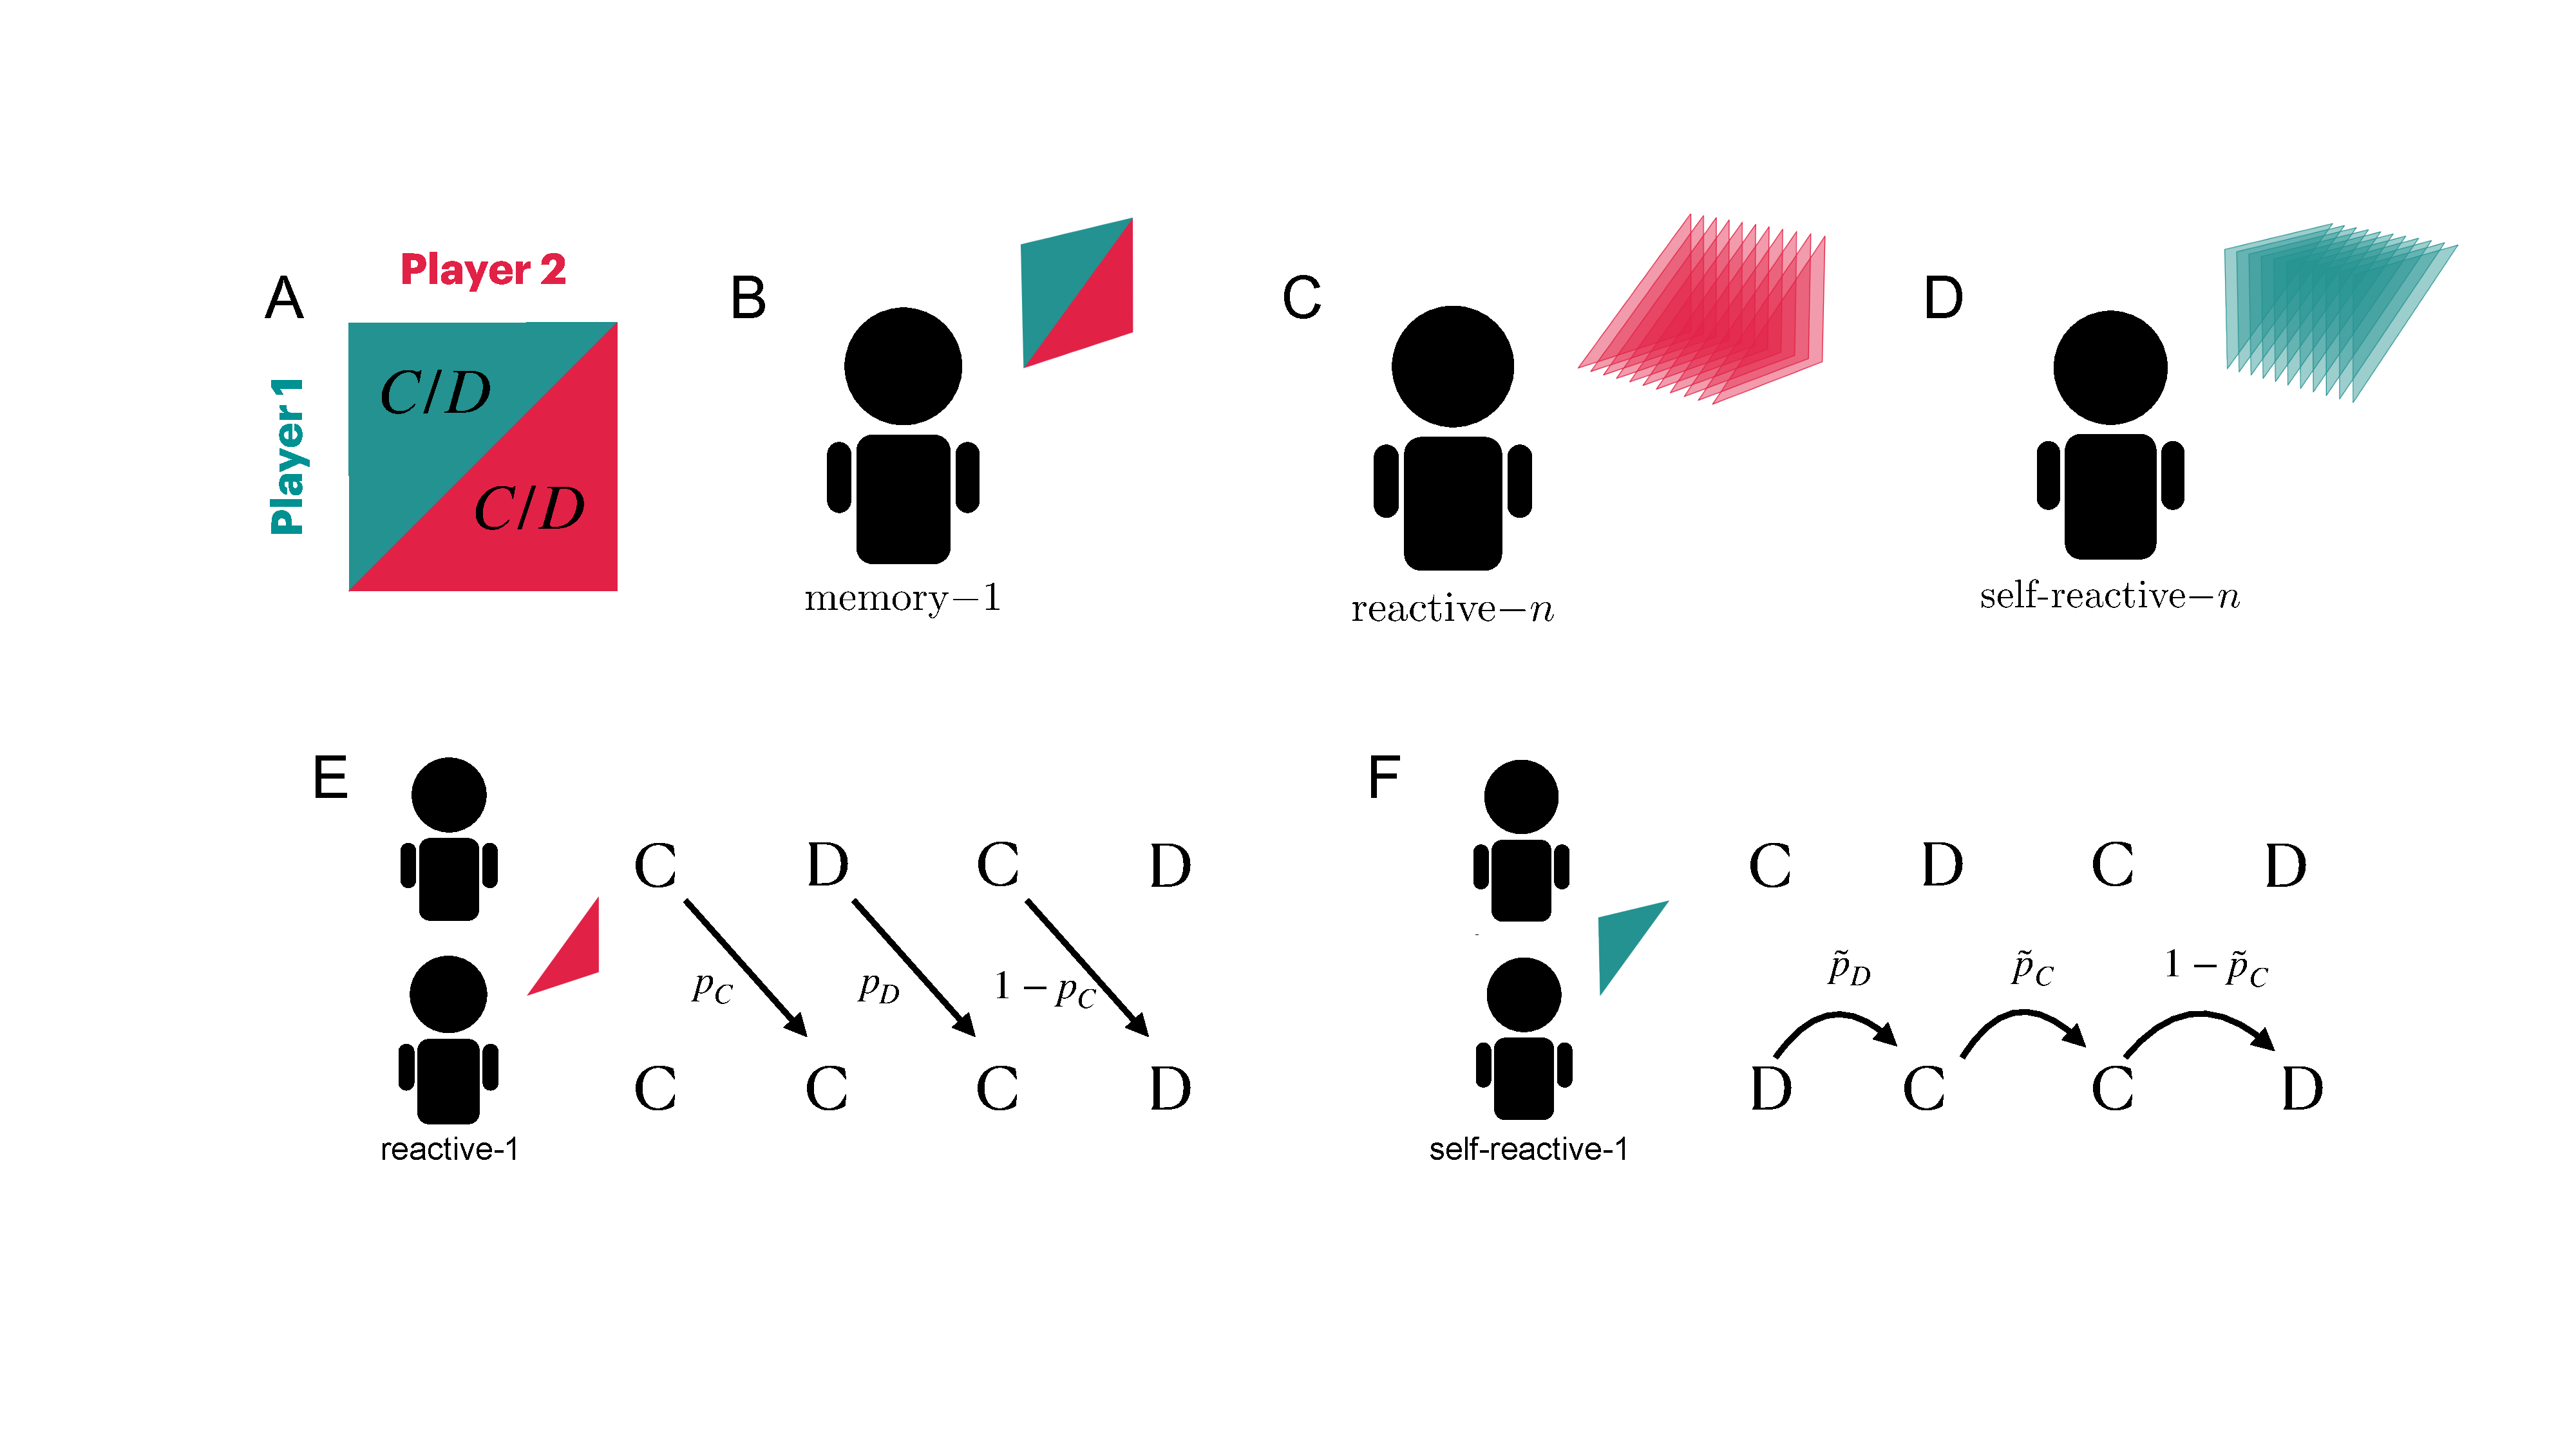
\includegraphics[width=0.75\textwidth]{figures/conceptual_figure_model.pdf}
  \caption{\textbf{The repeated prisoner's dilemma among players with finite memory.}
  \textbf{A,} In the repeated prisoner's dilemma, in each round two players independently decide whether to cooperate~($C$) or to defect~($D$). 
   \textbf{B,} When players adopt memory-1 strategies, their decisions depend on the outcome of the previous round. That is, they consider both their own and the co-player's previous action. 
   \textbf{C,} When players adopt a reactive-$n$ strategy, they make their decisions based on the co-player's actions during the past $n$ rounds. 
   \textbf{D,} A self-reactive-$n$ strategy is contingent on the player's own actions during the past $n$ rounds. 
   \textbf{E,} To illustrate these concepts, we show a game between an arbitrary player (top) and a player with a reactive-1 strategy (bottom). 
   Reactive-1 strategies can be represented as a vector  $\mathbf{p} \!=\! (p_C, p_D)$. 
   The entry $p_C$ is the probability of cooperating after the co-player cooperated in the previous round.
   The entry $p_D$ is the cooperation probability after the co-player defected. 
   \textbf{E,} Now, the bottom player adopts a self-reactive-1 strategy, $\mathbf{\tilde p}\!=\!(\tilde p_C, \tilde p_D)$. 
   Here, the bottom player's cooperation probabilities depend on their own previous action. }\label{fig:conceptual_figure_model}
\end{figure}


\begin{figure}[t]
  \centering
  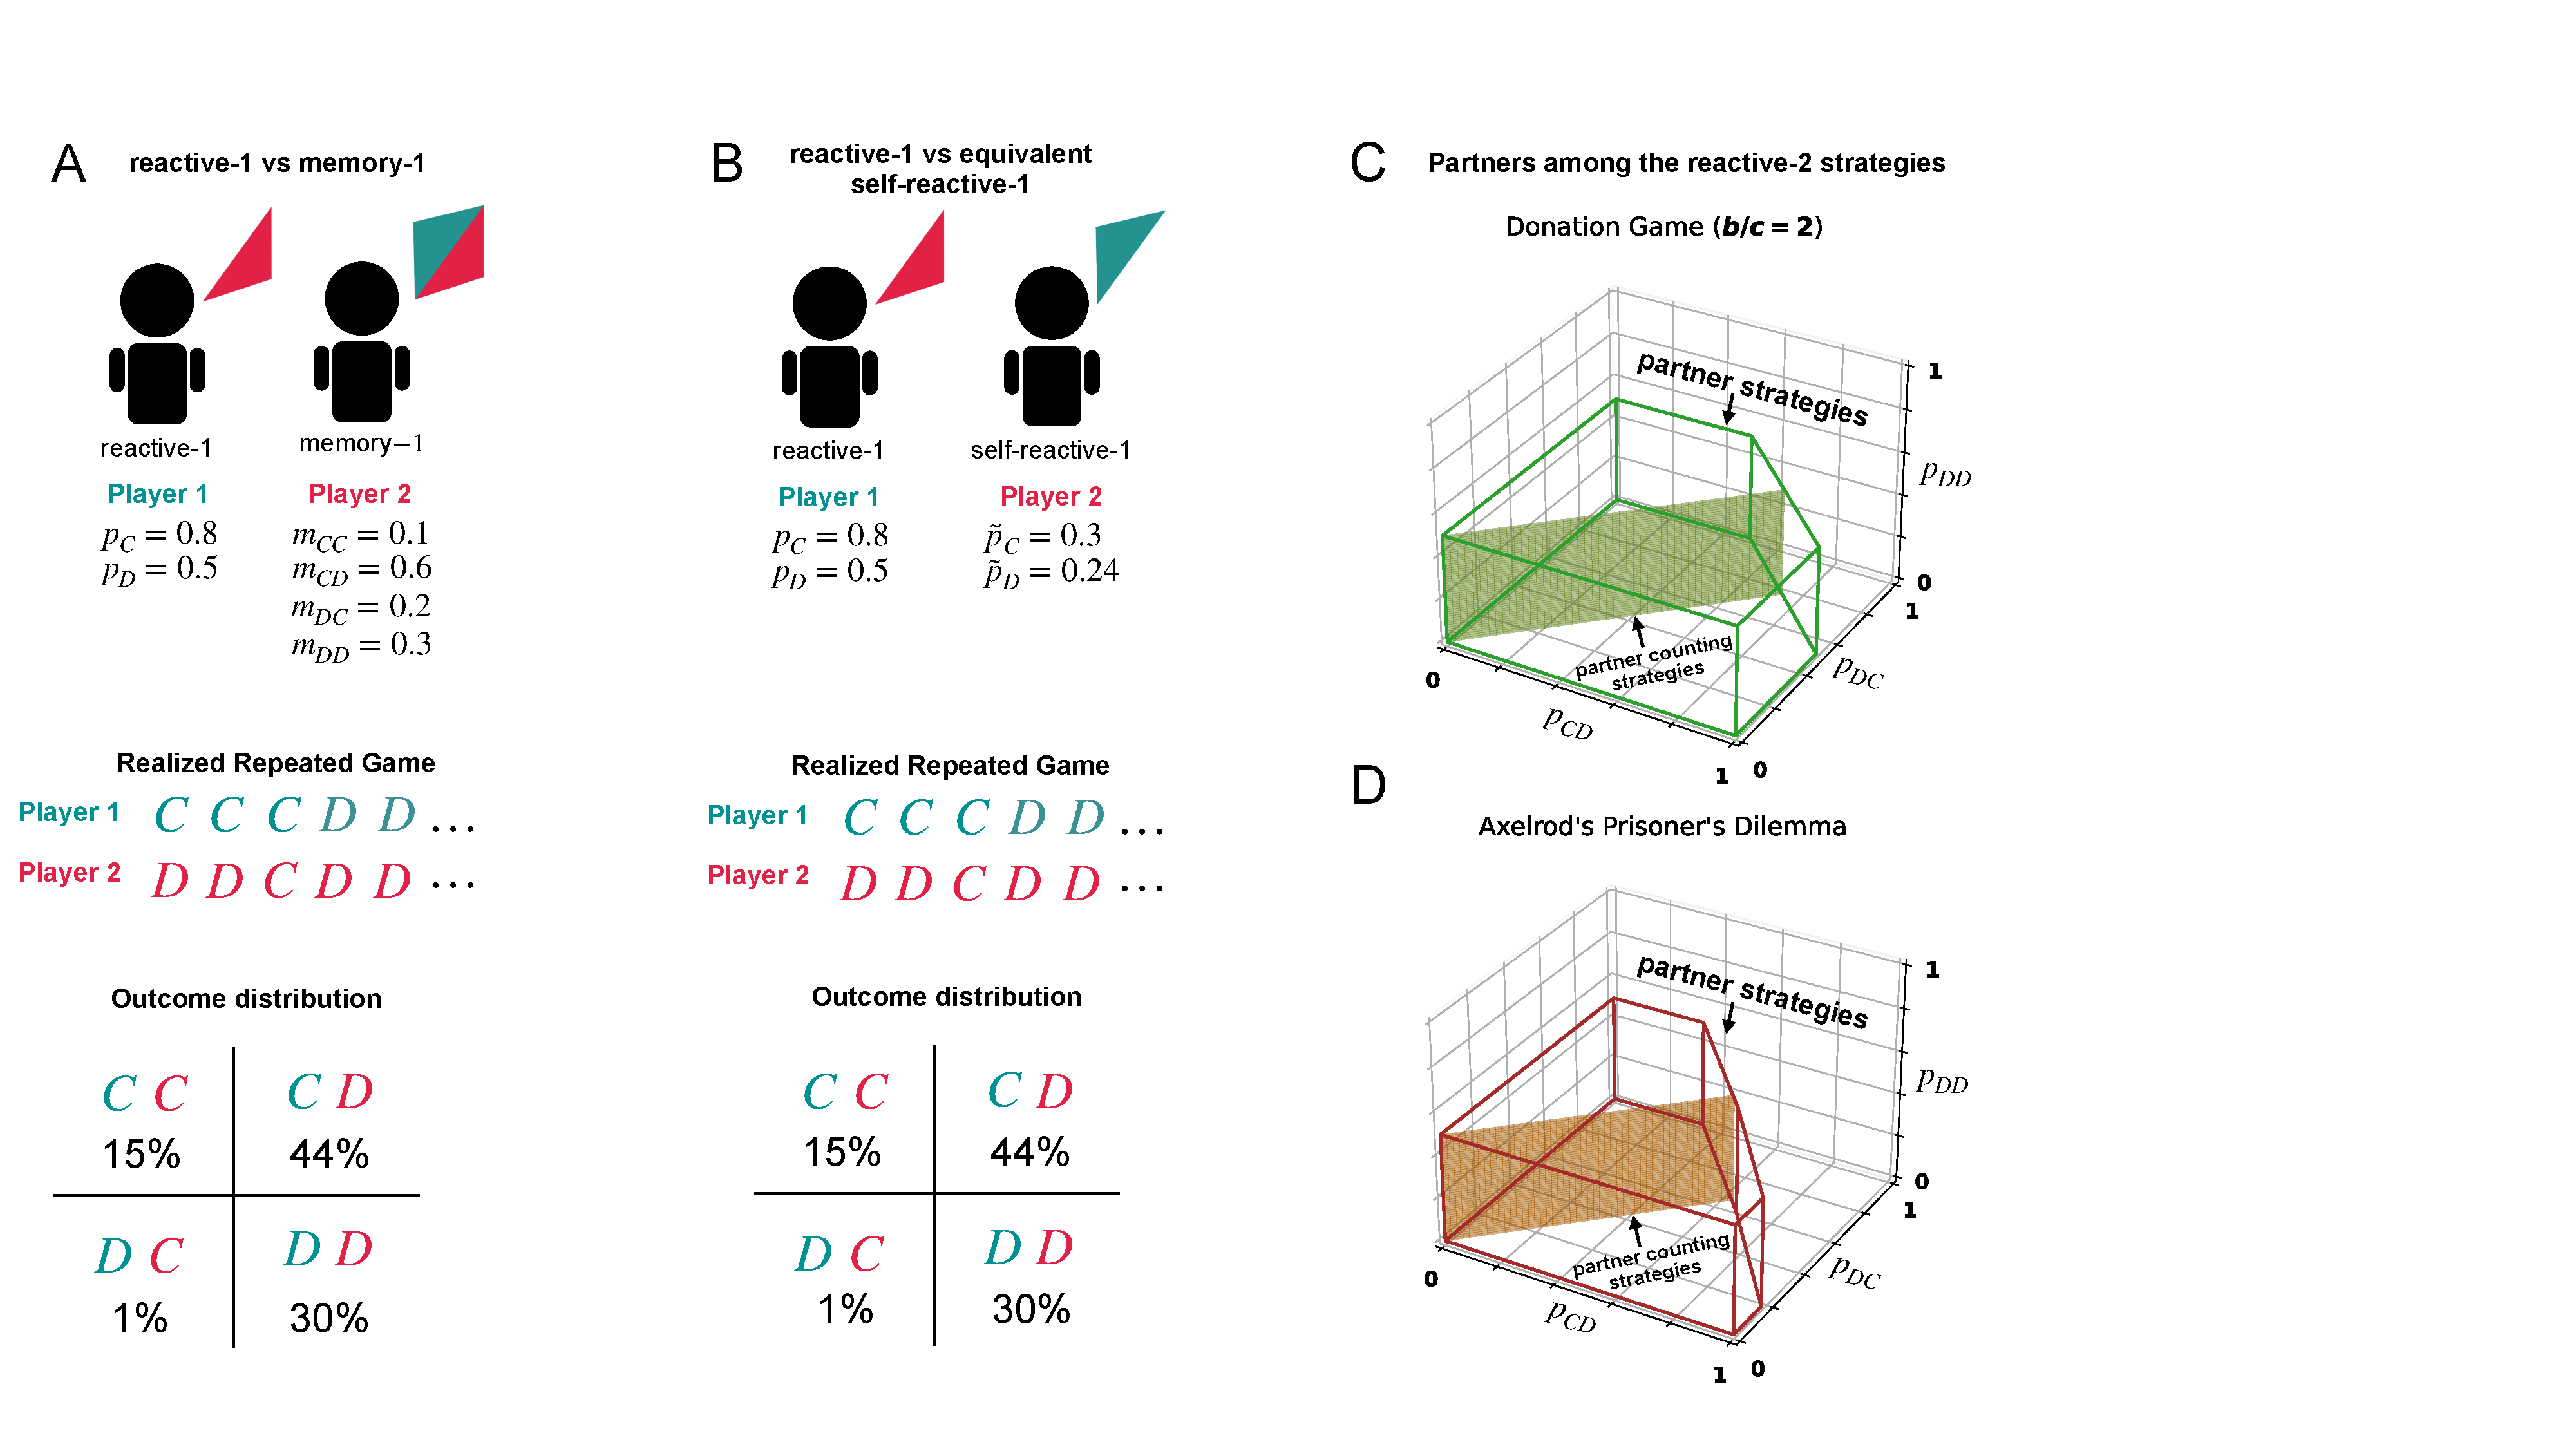
\includegraphics[width=\textwidth]{figures/conceptual_figure_results.pdf}
  \caption{
  \textbf{Characterizing the partners among the reactive-$n$ strategies.} 
{\bf A,B,} To characterize the reactive-$n$ partner strategies, we prove the following result. 
Suppose the focal player adopts a reactive-$n$ strategy. 
Then, for any strategy of the opponent (with arbitrary memory), one can find an associated self-reactive-$n$ strategy that yields the same payoffs. 
Here, we show an example where player~1 uses a reactive-1 strategy against player~2 with a memory-1 strategy. 
Our result implies that can switch to a well-defined self-reactive-1 strategy. 
This switch leaves the outcome distribution unchanged.
In both cases, players are equally likely to experience mutual cooperation, unilateral cooperation, or mutual defection in the long run. 
\textbf{C,} Based on this insight, we can explicitly characterize the reactive-2 partner strategies (with $p_{CC}\!=\!1$). 
Here, we represent the corresponding conditions~\eqref{eq:two_bit_conditions} for a donation game with $b/c\!=\!2$. 
Among the reactive-2 strategies, the counting strategies correspond to the subset with $p_{CD}\!=\!p_{DC}$. 
Counting strategies only depend on how often the co-player cooperated in the past, not on the timing of cooperation.
\textbf{D,} Similarly, we can also characterize the reactive-2 partner strategies for the general prisoner's dilemma. 
Here, we use the values of Axelrod~\citep{axelrod:AAAS:1981}.}\label{fig:conceptual_figure_results}
\end{figure}


\begin{figure}[t]
  \centering
  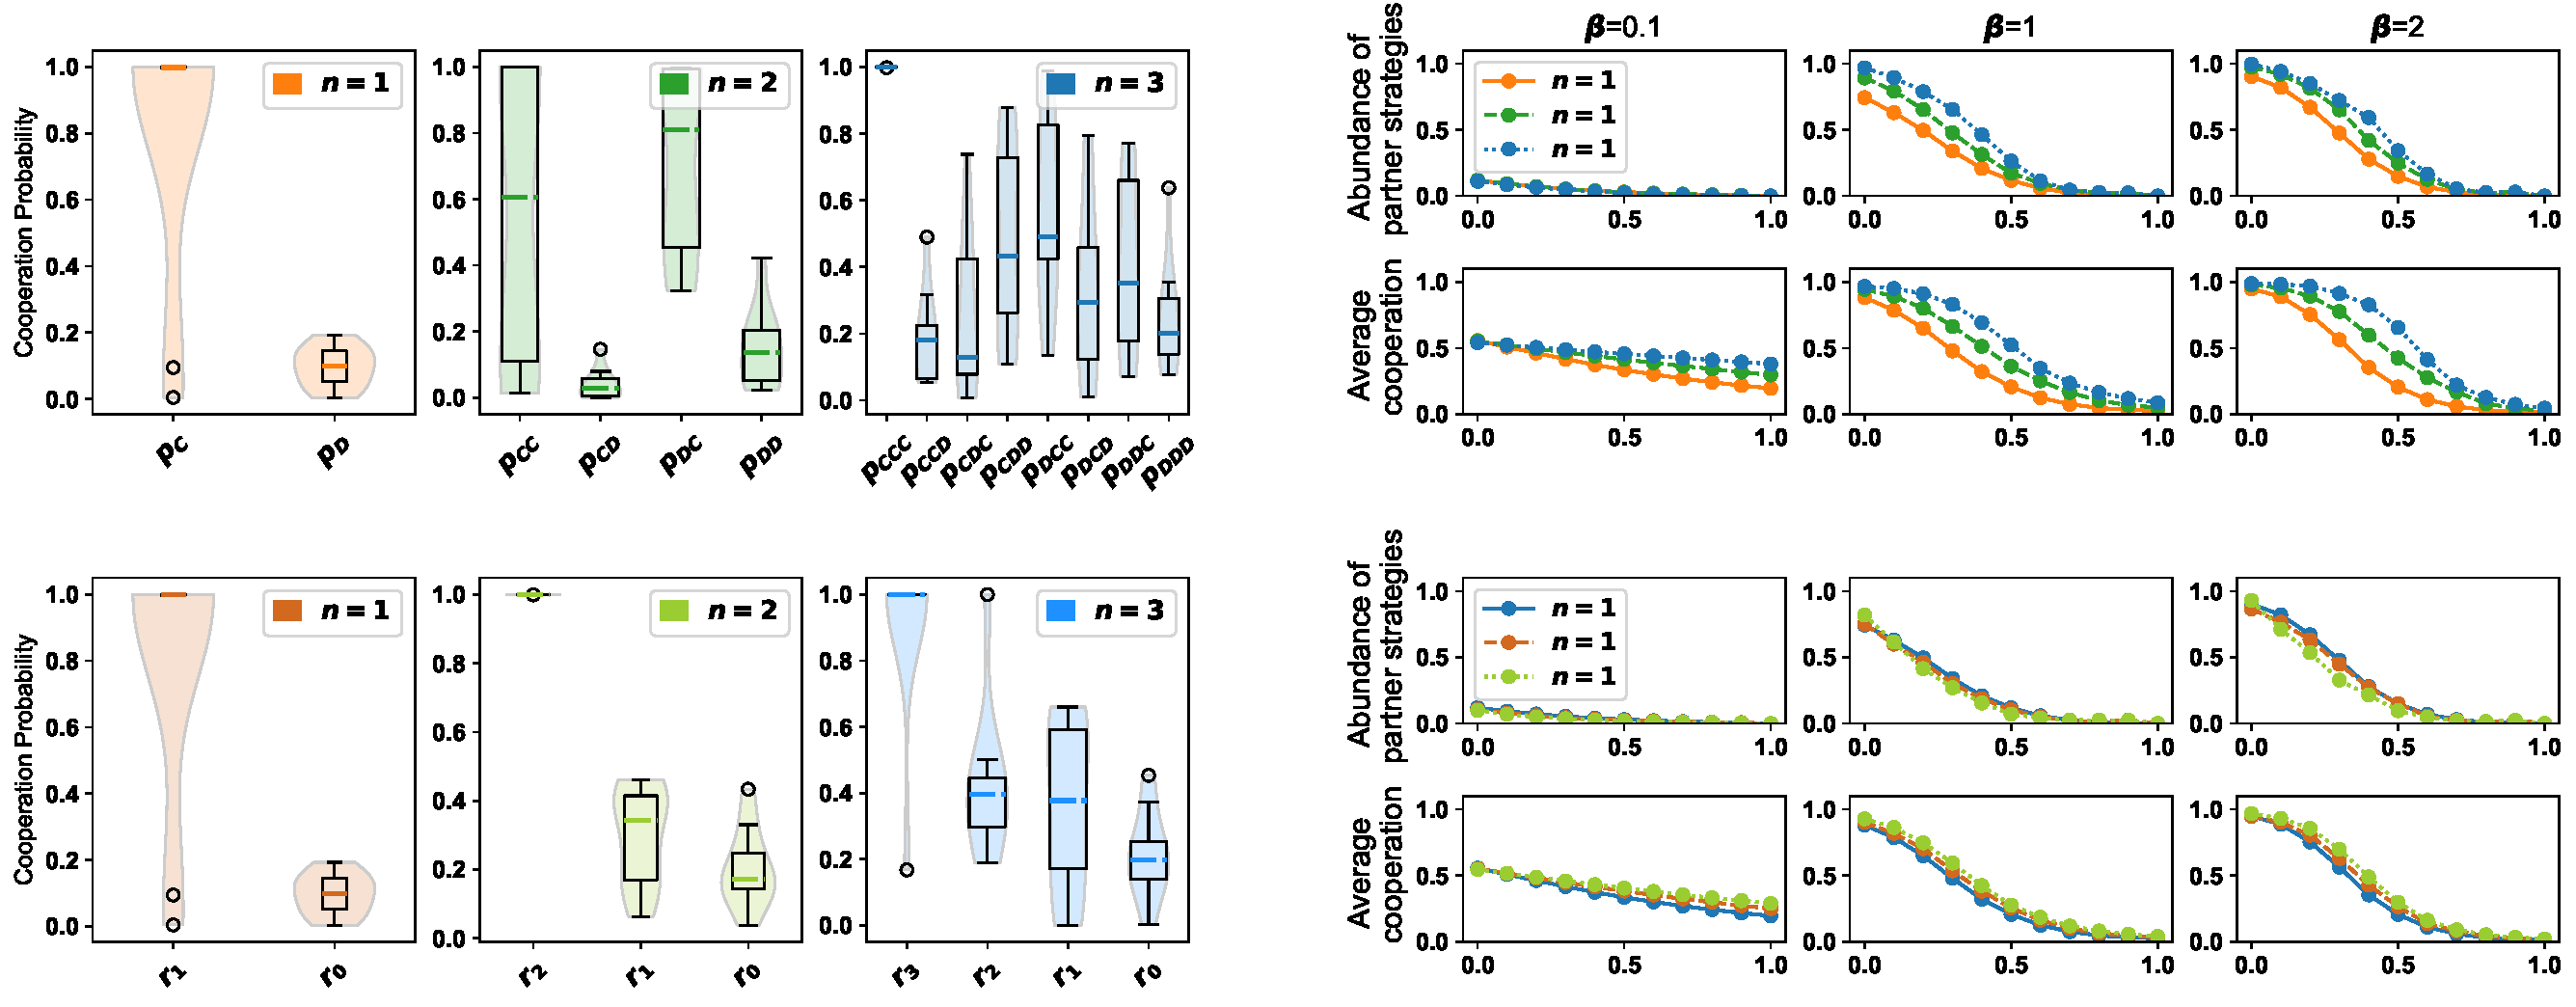
\includegraphics[width=\textwidth]{figures/abundant_strategies.pdf}
  \caption{\textbf{Evolutionary dynamics of reactive-$n$ strategies.}
  To explore the evolutionary dynamics among reactive-$n$ strategies, we run simulations based on the
  method of Imhof and Nowak~\cite{imhof:royal:2010}. 
  This method assumes rare mutations. 
  Every time a mutant strategy appears, it goes extinct or fixes before the arrival of the next mutant strategy. 
  {\bf A,B,} We consider ten independent simulations for reactive-$n$ strategies and for reactive-$n$ counting strategies. 
  For each simulation, we record the most abundant strategy (the strategy that resisted most mutants). 
  The respective average cooperation probabilities are in line with the conditions for partner strategies. 
  {\bf C,D,} With additional simulations, we explore the average abundance of partner strategies and the population's average cooperation rate for a range of different cooperation costs and selection strengths. 
  In all cases, we only observe high cooperation rates when partner strategies evolve. 
 Simulations are based on a donation game with \(b\!=\!1\),  \(c\!=\!.5\), and a selection strength parameter $\beta\!=\!1$, unless noted otherwise.     For $n$ equal to 1
  and 2, simulations are run for \(T\!=\! 10 ^ 7\) time steps. For $n\!=\!3$ we use \(T\!=\! 2 \!\cdot\!10 ^ 7\) time steps.}\label{fig:evolutionary_results}
\end{figure}


\end{document}




